\documentclass[uplatex, dvipdfmx, a4j,11pt]{jsarticle}
\usepackage[dvipdfmx]{graphicx}
\usepackage{lastpage}
\usepackage{fancyhdr}
\usepackage{listings}
\usepackage{jlisting}
\usepackage{xcolor}
\usepackage{url}
\usepackage{amsmath}

\makeatletter
\title{演習課題2}
\author{202310330 長田悠生}
\date{2024年6月18日}

\pagestyle{fancy}

\lstset{
    basicstyle = {\ttfamily}, % 基本的なフォントスタイル
    frame = {tbrl}, % 枠線の枠線。t: top, b: bottom, r: right, l: left
    breaklines = true, % 長い行の改行
    numbers = none, % 行番号の表示。left, right, none
    % stepnumber=1, % 行番号増分
    % numbersep=10pt, % 行番号と本文の間隔 デフォルト:10pt
    showspaces = false, % スペースの表示
    showstringspaces = false, % 文字列中のスペースの表示
    showtabs = false, % タブの表示
    keywordstyle = \color{blue}, % キーワードのスタイル。intやwhileなど
    commentstyle = {\color[HTML]{1AB91A}}, % コメントのスタイル
    identifierstyle = \color{black}, % 識別子のスタイル 関数名や変数名
    stringstyle = \color{brown}, % 文字列のスタイル
    captionpos = t % キャプションの位置 t: 上、b: 下
}

\lstdefinelanguage{Julia}
{
  keywordsprefix=\@,
  morekeywords={
    exit,whos,edit,load,is,isa,isequal,typeof,tuple,ntuple,uid,hash,finalizer,convert,promote,
    subtype,typemin,typemax,realmin,realmax,sizeof,eps,promote_type,method_exists,applicable,
    invoke,dlopen,dlsym,system,error,throw,assert,new,Inf,Nan,pi,im,begin,while,for,in,return,
    break,continue,macro,quote,let,if,elseif,else,try,catch,end,bitstype,ccall,do,using,module,
    import,export,importall,baremodule,immutable,local,global,const,Bool,Int,Int8,Int16,Int32,
    Int64,Uint,Uint8,Uint16,Uint32,Uint64,Float32,Float64,Complex64,Complex128,Any,Nothing,None,
    function,type,typealias,abstract
  },
  sensitive=true,
  morecomment=[l]{\#},
  morestring=[b]',
  morestring=[b]"
}
\renewcommand{\lstlistingname}{}

% headers & footers
\lhead{数値計算法 \@title 提出日:\@date\\\@author}
\chead{}
\rhead{}
\lfoot{}
\cfoot{\thepage/\pageref{LastPage}}
\rfoot{}
\renewcommand{\headrulewidth}{0pt}
\renewcommand{\footrulewidth}{0pt}
\makeatother

\begin{document}
\section*{課題1}
\subsection*{(1-1)}
\textmc{
  $f(x) = \frac{1}{25x^2 + 5x + 2}$をJuliaで書いたものを以下に示す。
}
\begin{lstlisting}[title={(1-1)}, label=code:in, language=Julia]
function f(x::Float64)
  return 1 / (25*x^2 + 5*x + 2)
end
\end{lstlisting}

\textmc{
  [-1, 1]の区間で等間隔に取った値と[0, $\pi$]の区間で$\theta_{i}$で等間隔に取ったときの$cos(\theta_{i})$の値を
  それぞれ補完点として補完多項式を求め、グラフにプロットした。
  $cos(\theta_{i})$の方が精度が良いことがわかる。
}

\begin{figure}[h]
  \begin{center}
    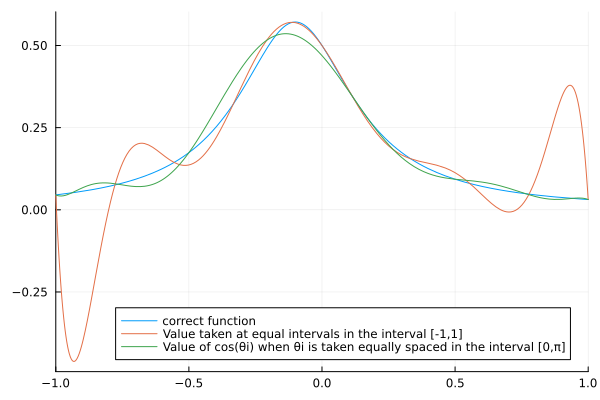
\includegraphics[width=100mm]{runge.png}
    \caption{Rungeの現象}
  \end{center}
\end{figure}

\textmc{
  以下が(1-1)のプログラムの全体である。
}

\begin{lstlisting}[title={(1-1)}, label=code:in, language=Julia]
module Runge

  using Plots
  using Polynomials

  function f(x::Float64)
    return 1 / (25*x^2 + 5*x + 2)
  end

  function runge_graph(start_point::Float64, end_point::Float64, cos_start_point::Float64, cos_end_point::Float64, point_quantity::Int64)
    x_r::Array{Float64} = range(start_point, end_point, point_quantity)
    range_r_poly = Polynomials.fit(x_r, f.(x_r))

    x_cos::Array{Float64} = cos.(range(cos_start_point, cos_end_point, point_quantity));
    range_cos_poly = Polynomials.fit(x_cos, f.(x_cos));

    correct_plot = Plots.plot(f, xlim=[-1.0, 1.0], label="correct function", legend=:bottomright)
    r_poly_plot = Plots.plot!(correct_plot, range_r_poly, xlim=[-1.0, 1.0], label="Value taken at equal intervals in the interval [-1,1]", legend=:bottomright)
    Plots.plot!(r_poly_plot, range_cos_poly, xlim=[-1.0, 1.0], label="Value of cos(θi) when θi is taken equally spaced in the interval [0,π]", legend=:bottomright)
    Plots.savefig("runge.png")
  end

end

using .Runge

Runge.runge_graph(-1.0, 1.0, 0.0, Float64(pi), 10)
\end{lstlisting}

\section*{課題2}
\subsection*{(2-1)}
\textmc{
  $x_{0}$から$x_{m-1}$を温度とする。温度のデータの数が9個で次関数で近似するので、
  $A =  \begin{pmatrix}
    x_{0}^0 & x_{1}^1 \\
    \vdots & \vdots \\
    x_{8}^0 & x_{8}^1\\
  \end{pmatrix}$を生成するプログラムをかけば良い。関数は以下の通りである。
}
\begin{lstlisting}[title={(2-1)}, label=code:in, language=Julia]
function make_a(temp::Array{Int64}, n::Int64)::Matrix{Float64}
  linage::Int64 = length(temp)
  a::Matrix{Float64} = [temp[i]^b for i in 1:linage, b in Float64(0):Float64(n)]
  return a
end
\end{lstlisting}

\subsection*{(2.2)}
\textmc{
  表1のデータをグラフにプロットした。
}
\begin{figure}[h]
  \begin{center}
    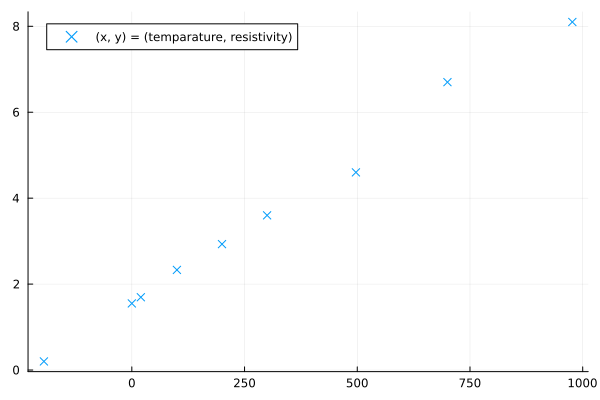
\includegraphics[width=100mm]{complete_plot.png}
    \caption{表1のデータ}
  \end{center}
\end{figure}
\textmc{
  以下が(2.2)のグラフの画像を生成する関数である。
}
\begin{lstlisting}[title={(2-2)}, label=code:in, language=Julia]
function complete_true_graph(temp::Array{Int64}, resistivity::Array{Float64})
  plot(temp, resistivity, markershape=:x, la=0.0, label="(x, y) = (temparature, resistivity)")
  savefig("complete_plot.png")
end
\end{lstlisting}

\newpage
\subsection*{(2.3)}
\textmc{
  以下が作成したグラフである。
}
\begin{figure}[h]
  \begin{center}
    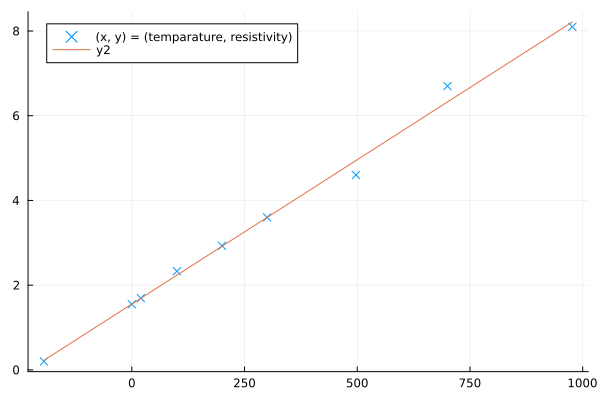
\includegraphics[width=100mm]{complete.png}
    \caption{(2.3)}
  \end{center}
\end{figure}
\textmc{
  以下がグラフを作成すために書いたプログラムである。
}
\begin{lstlisting}[title={(2-3)}, label=code:in, language=Julia]
module Complete

  using Plots
  using LinearAlgebra

  function make_a(temp::Array{Int64}, n::Int64)::Matrix{Float64}
    linage::Int64 = length(temp)
    a::Matrix{Float64} = [temp[i]^b for i in 1:linage, b in Float64(0):Float64(n)]
    return a
  end

  function gen_a_b(a::Matrix{Float64}, resistivity::Array{Float64})::Vector{Float64}
    Q0::LinearAlgebra.QRCompactWYQ{Float64, Matrix{Float64}, Matrix{Float64}}, R::Matrix{Float64} = LinearAlgebra.qr(a)
    Q::Matrix{Float64} = Matrix(Q0)
    c::Vector{Float64} = inv(R) * Q' * resistivity
    return c
  end

  function complete_graph(temp::Array{Int64}, resistivity::Array{Float64}, a::Matrix{Float64})
    c::Vector{Float64} = gen_a_b(a, resistivity)
    function f(x)
      return c[2] * x + c[1]
    end
    true_graph = Plots.plot(temp, resistivity, markershape=:x, la=0.0,  label="(x, y) = (temparature, resistivity)")
    Plots.plot!(true_graph, f)
    savefig("complete.png")
  end

end

using .Complete

temp::Array{Int64} = [-195, 0, 20, 100, 200, 300, 497, 700, 977]
resistivity::Array{Float64} = [0.2,	1.55,	1.694, 2.33, 2.93, 3.6, 4.6, 6.7, 8.1]
a::Matrix{Float64} = Complete.make_a(temp, 1)
Complete.complete_graph(temp, resistivity, a)

\end{lstlisting}

\subsection*{(2.4-1)}
\textmc{
  $y=ax+b$の$a$と$b$はわかっているのので、$x$または$y$を代入すれば、もう一方の未知数は求めることができる。\\
  400度は$x$なので$y$を計算するプログラムに$400.0$を代入すれば良い。\\
  以下がyを推測するために必要なプログラムである。\\
}
\begin{lstlisting}[title={(2-3)}, label=code:in, language=Julia]
  module Complete

  using Plots
  using LinearAlgebra

  function make_a(temp::Array{Int64}, n::Int64)::Matrix{Float64}
    linage::Int64 = length(temp)
    a::Matrix{Float64} = [temp[i]^b for i in 1:linage, b in Float64(0):Float64(n)]
    return a
  end

  function gen_a_b(a::Matrix{Float64}, resistivity::Array{Float64})::Vector{Float64}
    Q0::LinearAlgebra.QRCompactWYQ{Float64, Matrix{Float64}, Matrix{Float64}}, R::Matrix{Float64} = LinearAlgebra.qr(a)
    Q::Matrix{Float64} = Matrix(Q0)
    c::Vector{Float64} = inv(R) * Q' * resistivity
    return c
  end

  function guess_y(x::Float64, c::Vector{Float64})
    return c[2] * x + c[1] 
  end

  function guess_x(y::Float64, c::Vector{Float64})
    return (y - c[1]) / c[2]
  end

end

using .Complete

temp::Array{Int64} = [-195, 0, 20, 100, 200, 300, 497, 700, 977]
resistivity::Array{Float64} = [0.2,	1.55,	1.694, 2.33, 2.93, 3.6, 4.6, 6.7, 8.1]

a::Matrix{Float64} = Complete.make_a(temp, 1)
c::Vector{Float64} = Complete.gen_a_b(a, resistivity)

temp_1 = Complete.guess_x(2.00, c)
println(temp_1)

\end{lstlisting}
\textmc{
  プログラムの実行結果を以下に示す。
}
\begin{lstlisting}[title={(2.4-1の実行結果)}, label=code:in, language=sh]
$ julia --project ./src/complete2-41.jl
65.33316000373105
\end{lstlisting}

\textmc{
  2.00は、yなのでxを計算するプログラムに2.00を代入すれば良い。
  以下がxを推測するために必要なプログラムである。
}
\begin{lstlisting}[title={(2.4-2)}, label=code:in, language=Julia]
  module Complete

  using Plots
  using LinearAlgebra

  function make_a(temp::Array{Int64}, n::Int64)::Matrix{Float64}
    linage::Int64 = length(temp)
    a::Matrix{Float64} = [temp[i]^b for i in 1:linage, b in Float64(0):Float64(n)]
    return a
  end

  function gen_a_b(a::Matrix{Float64}, resistivity::Array{Float64})::Vector{Float64}
    Q0::LinearAlgebra.QRCompactWYQ{Float64, Matrix{Float64}, Matrix{Float64}}, R::Matrix{Float64} = LinearAlgebra.qr(a)
    Q::Matrix{Float64} = Matrix(Q0)
    c::Vector{Float64} = inv(R) * Q' * resistivity
    return c
  end

  function guess_y(x::Float64, c::Vector{Float64})
    return c[2] * x + c[1]
  end

  function guess_x(y::Float64, c::Vector{Float64})
    return (y - c[1]) / c[2]
  end

end

using .Complete

temp::Array{Int64} = [-195, 0, 20, 100, 200, 300, 497, 700, 977]
resistivity::Array{Float64} = [0.2,	1.55,	1.694, 2.33, 2.93, 3.6, 4.6, 6.7, 8.1]

a::Matrix{Float64} = Complete.make_a(temp, 1)
c::Vector{Float64} = Complete.gen_a_b(a, resistivity)

resistivity_1 = Complete.guess_y(400.0, c)
println(resistivity_1)
\end{lstlisting}

\newpage
\section*{課題3}
\subsection*{(3.1)}
\textmc{
  $n=1, \cdots , 15$までのmysin関数の計算結果を$sin\left(\frac{\pi}{4}\right)$の結果との相対誤差を取ってグラフにプロットしたものを以下に示す。
}
\begin{figure}[h]
  \begin{center}
    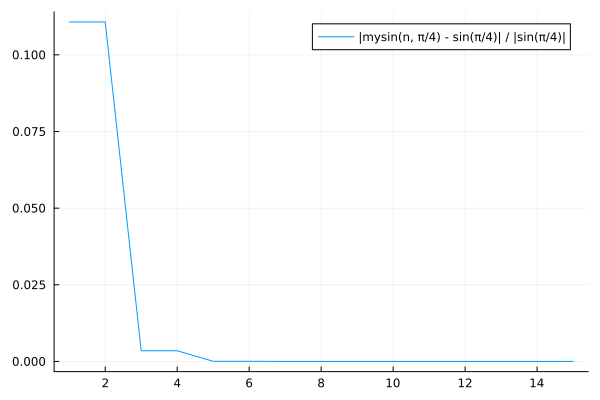
\includegraphics[width=100mm]{mysin.png}
    \caption{(2.3)}
  \end{center}
\end{figure}
\subsection*{(3.2)}
\textmc{
  $n=1, 3, 5, 7$のときの区間$[0, \pi]$のグラフを以下に示す。\\
  $n$の値が大きくなればなるほど、精度が良くなっていることがわかる。
}
\begin{figure}[h]
  \begin{center}
    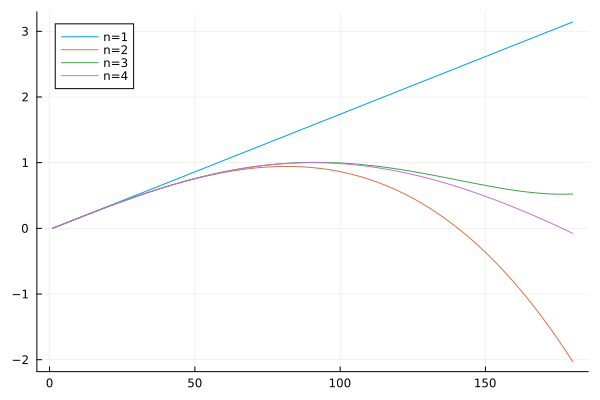
\includegraphics[width=100mm]{sin_maclaurin.png}
    \caption{(2.3)}
  \end{center}
\end{figure}

\textmc{
  課題3の全体のプログラムは以下のようになっている。
}
\begin{lstlisting}[title={(2-3)}, label=code:in, language=Julia]
  module Sin

  using Plots

  function mysin(n::Int64, x::Float64)::Float64
    xn = x
    P  = x
    k  = ceil(n / 2) - 1
    for i = 1:k
      r  = ((-1) / ( (2*i) * (2*i + 1))) * x^2
      xn = xn * r
      P  = P + xn
    end
    return P
  end

  function sin_maclaurin(power_start::Int64, power_end::Int64, x::Float64)
    p_array::Array{Float64} = zeros(Float64, 0)
    correct::Float64 = sin(x)
    for n=range(power_start, power_end, (power_end - power_start + 1))
      p::Float64 = mysin(Int64(n), x)
      #相対誤差の配列
      push!(p_array, abs(p - correct) / abs(correct))
    end
    Plots.plot(power_start:power_end, p_array, label="|mysin(n, π/4) - sin(π/4)| / |sin(π/4)|")
    savefig("mysin.png")
  end

  function sin_maclaurin_data(start_point::Float64, end_point::Float64, step_point::Int64, n::Int64)::Array{Float64}
    sin_array::Array{Float64} = zeros(Float64, 0)
    for x=range(start_point, end_point, step_point)
      sin_point::Float64 = mysin(n, x)
      push!(sin_array, sin_point)
    end
    return sin_array
  end

  function sin_maclaurin_graph(start_point::Float64, end_point::Float64, step_point::Int64, n_array::Array{Int64})
    for n=1:length(n_array)
      sin_array = sin_maclaurin_data(start_point, end_point, step_point, n_array[n])
      if n == 1
        Plots.plot(1:step_point, sin_array, label="n=$n")
      else
        Plots.plot!(1:step_point, sin_array, label="n=$n")
      end
    end
    savefig("sin_maclaurin.png")
  end

end

using .Sin
using Plots

#(3.1)
const x::Float64 = pi / 4
Sin.sin_maclaurin(1, 15, x)

#(3.2)
Sin.sin_maclaurin_graph(0.0, Float64(pi), 180, [1, 3, 5, 7])
\end{lstlisting}
\subsection*{(3.3)}
\textmc{
  マクローリン展開を第n項までで止めた場合、$\frac{f^{(n+1)(c)}}{(n+1)!}x^{n+1}$の誤差が発生する。
  $n$を大きくしていくと誤差は小さくなっていくが、$x^{n+1}$の増加量に対しての$(n+1)!$の増加量が小さくなってしまう。
  そのため、次数$n$を十分に大きくしても多項式の値の計算に寄与しなくなる。
}

\section*{課題4}
\subsection*{(4.1)}
\textmc{
  以下がmyexpの関数である。
}
\begin{lstlisting}[title={(4.1)}, label=code:in, language=Julia]
function myexp(n::Int64, x::Float64)::Float64
  xn::Float64 = 1.0
  P::Float64 = 1.0
  if n == 0
  else
    for k = 0:(n-1)
      r = x / (k+1)
      xn = xn * r
      P = P + xn
    end
  end
  return P
end
\end{lstlisting}
\subsection*{(4.2)}
\textmc{
  以下がmyexp2の関数である。
}
\begin{lstlisting}[title={(4.2)}, label=code:in, language=Julia]
function myexp2(n::Int64, x::Float64)::Float64
  P::Float64 = 0.0
  if x > 0
    P = myexp(n, x)
  else
    P = (1 / myexp(n, -x))
  end
  return P
end
\end{lstlisting}
\subsection*{(4.3)}
\textmc{
  以下がmyexp3の関数である。
}
\begin{lstlisting}[title={(4.2)}, label=code:in, language=Julia]
function myexp3(n::Int64, x::Float64)::Float64
  #整数部
  x_int::Int64 = convert(Int, floor(x))
  #小数部
  x_decimal::Float64 = x - x_int
  #整数部の計算
  #result_int::Float64=exp(x_int)
  result_int::Float64 = 1.0
  if x_int > 0
    for i=1:x_int
      result_int = result_int * ℯ
    end
  elseif x_int == 0
  else
    for i=1:-x_int
        result_int = result_int * ℯ
    end
    result_int = 1 / result_int
  end
  #小数部の計算
  P::Float64 = myexp(n, x_decimal)
  return (result_int * P)
end
\end{lstlisting}

\newpage
\subsection*{(4.4)}
\begin{figure}[h]
  \begin{center}
    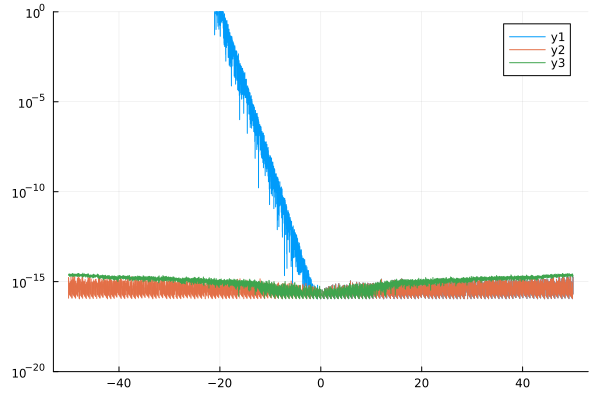
\includegraphics[width=100mm]{exp200_50.png}
    \caption{n=200, 区間 [-50, 50]}
  \end{center}
\end{figure}
\begin{figure}[h]
  \begin{center}
    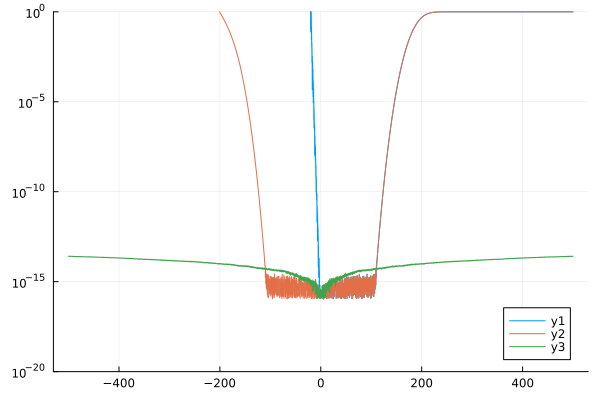
\includegraphics[width=100mm]{exp200_500.png}
    \caption{n=200, 区間 [-500, 500]}
  \end{center}
\end{figure}
\begin{figure}[h]
  \begin{center}
    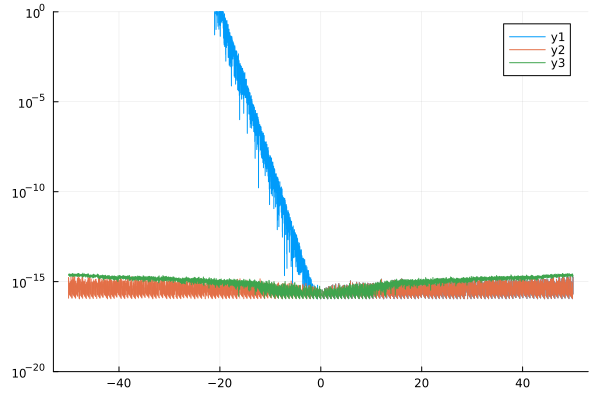
\includegraphics[width=100mm]{exp1000_50.png}
    \caption{n=1000, 区間 [-50, 50]}
  \end{center}
\end{figure}
\begin{figure}[h]
  \begin{center}
    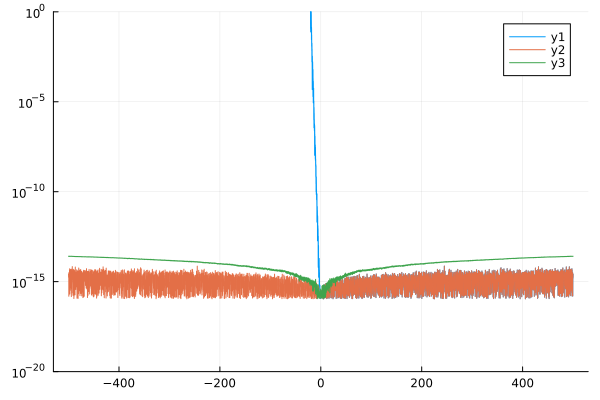
\includegraphics[width=100mm]{exp1000_500.png}
    \caption{n=1000, 区間 [-500, 500]}
  \end{center}
\end{figure}

\newpage
\textmc{
  課題4の全体のプログラムを以下に示す。
}
\begin{lstlisting}[title={課題4}, label=code:in, language=Julia]
module Exp

  using Plots

  function myexp(n::Int64, x::Float64)::Float64
    xn::Float64 = 1.0
    P::Float64 = 1.0
    if n == 0
    else
      for k = 0:(n-1)
        r = x / (k+1)
        xn = xn * r
        P = P + xn
      end
    end
    return P
  end

  function myexp2(n::Int64, x::Float64)::Float64
    P::Float64 = 0.0
    if x > 0
      P = myexp(n, x)
    else
      P = (1 / myexp(n, -x))
    end
    return P
  end

  function myexp3(n::Int64, x::Float64)::Float64
    #整数部
    x_int::Int64 = convert(Int, floor(x))
    #小数部
    x_decimal::Float64 = x - x_int
    #整数部の計算
    #result_int::Float64=exp(x_int)
    result_int::Float64 = 1.0
    if x_int > 0
      for i=1:x_int
        result_int = result_int * ℯ
      end
    elseif x_int == 0
    else
      for i=1:-x_int
         result_int = result_int * ℯ
      end
      result_int = 1 / result_int
    end
    #小数部の計算
    P::Float64 = myexp(n, x_decimal)
    return (result_int * P)
  end

  function exp_relative_error_data(n::Int64, start_point::Float64, end_point::Float64, point_quantity::Int64)::Tuple{Array{Float64}, Array{Float64}, Array{Float64}}
    myexp_arrary::Array{Float64} = zeros(Float64, 0) 
    myexp2_arrary::Array{Float64} = zeros(Float64, 0) 
    myexp3_arrary::Array{Float64} = zeros(Float64, 0) 
    for x in range(start_point, end_point, point_quantity)
      correct_point::Float64 = exp(x)
      exp_relative_error::Float64 = abs(myexp(n, x) - correct_point) / abs(correct_point)
      exp2_relative_error::Float64 = abs(myexp2(n, x) - correct_point) / abs(correct_point)
      exp3_relative_error::Float64 = abs(myexp3(n, x) - correct_point) / abs(correct_point)

      push!(myexp_arrary, exp_relative_error)
      push!(myexp2_arrary, exp2_relative_error)
      push!(myexp3_arrary, exp3_relative_error)
    end
    return tuple(myexp_arrary, myexp2_arrary, myexp3_arrary)
  end

  function exp_graph(n::Int64, start_point::Float64, end_point::Float64, point_quantity::Int64, png::String)
    myexp_arrary::Array{Float64}, myexp2_arrary::Array{Float64}, myexp3_arrary::Array{Float64} = exp_relative_error_data(n, start_point, end_point, point_quantity) 

    Plots.plot(range(start_point, end_point, point_quantity), myexp_arrary, ylim=[10^(-20), 1.0], yaxis=:log)
    Plots.plot!(range(start_point, end_point, point_quantity), myexp2_arrary, ylim=[10^(-20), 1.0], yaxis=:log)
    Plots.plot!(range(start_point, end_point, point_quantity), myexp3_arrary, ylim=[10^(-20), 1.0], yaxis=:log)
    savefig("$png")
  end

end

import .Exp

hello::Float64 = Exp.myexp(10, -3.14)

println("答え: $(exp(-3.14)), マクローリン: $hello")

hello2::Float64 = Exp.myexp2(10, -3.14)

println("答え: $(exp(-3.14)), マクローリン: $hello2")

hello3::Float64 = Exp.myexp3(10, -3.14)

println("答え: $(exp(-3.14)), マクローリン: $hello3")

a, b, c = Exp.exp_relative_error_data(200, -50.0, 50.0, 101)

println("myexp = $a, myexp2 = $b, myexp3 = $c")

Exp.exp_graph(200, -50.0, 50.0, 10000, "exp200_50.png")
Exp.exp_graph(200, -500.0, 500.0, 10000, "exp200_500.png")
Exp.exp_graph(1000, -50.0, 50.0, 10000, "exp1000_50.png")
Exp.exp_graph(1000, -500.0, 500.0, 10000, "ex1000_500.png")

\end{lstlisting}

\end{document}
